\setcounter{chapter}{0}
\chapter{Vectors}

\section{The Geometry and Algebra of Vectors}

\textbf{Vector}: a directed line segment that corresponds to a displacement from
one point $A$ to another point $B$.

\subsection*{Vector Addition}
$$\*{u+v}=[u_1+v_1, u_2+v_2]$$

\subsection*{Example}
If $\*{u}=[3,-1]$ and $\*{v}=[1,4]$ compute and draw $\*{u+v}$

\subsection*{Solution}
We compute $\*{u + v} = [3+1, -1+4] = [4,3]$
\begin{center}
    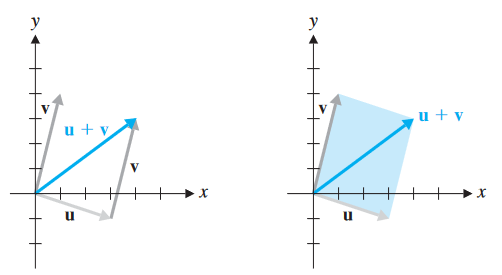
\includegraphics[scale=0.7]{example1-1-1.png}
\end{center}

\subsection*{Scalar Multiplication}
$$c\*{v}=c[\*{v}_1,\*{v}_2]=[c\*{v}_1, c\*{v}_2]$$

\subsection*{Example}
If $\*{v} = [2,-4]$, compute and draw $2\*{v}$, $\frac{1}{2}\*{v}$, and $-2\*{v}$

\subsection*{Solution}
\begin{enumerate}
    \item[] $2\*{v} = [2(-2),2(4)] = [-4,8]$
    \item[] $\frac{1}{2}\*{v} = [\frac{1}{2}(-2),\frac{1}{2}(4)] = [1,-2]$
    \item[] $-2\*{v} = [-2(-2),-2(4)] = [4,-8]$
\end{enumerate}
\begin{center}
    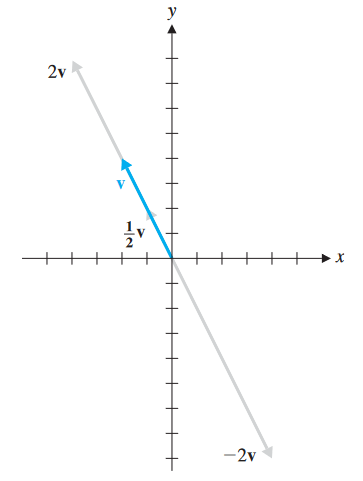
\includegraphics[scale=0.5]{example1-2-1.png}
\end{center}

\subsection*{Algebraic Properties of Vectors in $\mathbb{R}^n$}
Let \textbf{u}, \textbf{v}, and \textbf{w} be vectors in $\mathbb{R}^n$ and let
$c$ and $d$ be scalars. Then
\begin{enumerate}[(a)]
    \item $\*{u+v=v+u}$
    \item $\*{(u + v) + w = u + (v + w)}$
    \item $\*{u + 0 = u}$
    \item $\*{u + (-u) = 0}$
    \item $c\*{(u + v)=}c\*{u}+c\*{v}$
    \item $(c+d)\*{u}=c\*{u}+d\*{u}$
    \item $c(d\*{u})=(cd)\*{u}$
    \item $1\*{u}=\*{u}$
\end{enumerate}

A vector $\*{v}$ is a \textbf{linear combination} of vectors $\*{v_1,v_2,\dots,v_k}$ if
there are scalars $c_1,c_2, \dots , c_k$ such that $\*{v}=c_1\*{v}_1,c_2\*{v}_2,\dots,c_k\*{v}_k$.
The scalars $c_1,c_2,\dots,c_k$ are called the coefficients of the linear combination.

\section{Length and Angle: The Dot Product}

\subsection*{The Dot Product}
If
$$\vec{u}=\begin{bmatrix}
        u_1 \\ u_2 \\ \dots \\ u_n
    \end{bmatrix} \quad \text{and} \quad
    \vec{v}=\begin{bmatrix}
        v_1 \\ v_2 \\ \dots \\ v_n
    \end{bmatrix}$$
then the dot product of $\*{u \cdot v} = u_1v_1 + u_2v_2 + \dots + u_nv_n$

\subsection*{Example}
Compute $\*{u \cdot v}$ when
$$\vec{u}=\begin{bmatrix}
        1 \\ 2 \\ -3
    \end{bmatrix} \quad \text{and} \quad
    \vec{v}=\begin{bmatrix}
        -3 \\ 5 \\ 2
    \end{bmatrix}$$

\subsection*{Solution}
$$\*{u \cdot v} = 1 \cdot (-3) + 2 \cdot 5 + (-3) \cdot 2 = 1$$

\subsection*{Theorem}
Let \textbf{u}, \textbf{v}, and \textbf{w} be vectors in $\mathbb{R}^n$ and let $c$
be a scalar. Then
\begin{enumerate}[(a)]
    \item $\*{u\cdot v=v\cdot u}$
    \item $\*{(u\cdot v)\cdot w=u\cdot(v\cdot w)}$
    \item $(c\*u)\cdot\*v=c(\*{u\cdot v})$
    \item $\*{u\cdot u}\geq 0$ and $\*{u\cdot u}=0$ if and only if $\*u=0$
\end{enumerate}

The \textbf{length} (or \textbf{norm}) of a vector \textbf{v} in $\mathbb{R}^n$ is the
nonnegative scalar $\Vert\*v\Vert$ defined by
$$\Vert\vec{v}\Vert=\sqrt{\vec{v}\cdot\vec{v}}=\sqrt{v_1^2+v_2^2+\dots+v_n^2}$$

\subsection*{Theorem}
Let \textbf{v} be a vector in $\mathbb{R}^n$ and let $c$ be a scalar. Then
\begin{enumerate}[(a)]
    \item $\Vert\*v\Vert=0$ if and only if $\*v=0$
    \item $\Vert c\*v\Vert=|c|\Vert\*v\Vert$
\end{enumerate}

\subsection*{Cauchy-Schwarz Inequality}
For all vectors \textbf{u} and \textbf{v} in $\mathbb{R}^n$,
$$\Vert\*{u\cdot v}\Vert\leq\Vert\*u\Vert \Vert\*v\Vert$$

\subsection*{The Triangle Inequality}
For all vectors \textbf{u} and \textbf{v} in $\mathbb{R}^n$,
$$\Vert\*{u+v}\Vert\leq\Vert\*u\Vert+\Vert\*v\Vert$$

\subsection*{Proof}
\begin{enumerate}
    \item[] $\Vert\*{u+v}\Vert^2=\*{(u+v)\cdot(u+v)}$
    \item[] $=\*{u\cdot u}+2(\*{u\cdot v})+\*{v\cdot v}$
    \item[] $\leq\Vert\*u\Vert^2+2|\*{u\cdot v}|+\Vert\*v\Vert^2$
    \item[] $\leq\Vert\*u\Vert^2+2\Vert\*u\Vert \Vert\*v\Vert+\Vert\*v\Vert^2$
    \item[] $=(\Vert\*u\Vert+\Vert\*v\Vert)^2$
\end{enumerate}

For nonzero vectors \textbf{u} and \textbf{v} in $\mathbb{R}^n$,
$$\cos{\theta}=\frac{\vec{u}\cdot\vec{v}}{\Vert\vec{u}\Vert \Vert\vec{v}\Vert}$$

Two vectors \textbf{u} and \textbf{v} are \textbf{orthogonal} to each other if
$\*{u\cdot v} = 0$

If \textbf{u} and \textbf{v} are vectors in $\mathbb{R}^n$ and $u\neq 0$, then the
\textbf{projection of v onto u} is the vector $\text{proj}_u(\*v)$ defined by
$$\text{proj}_u(\vec{v})=\frac{(\vec{u}\cdot\vec{v})}{\vec{u}\cdot\vec{u}}\vec{u}$$

\subsection*{Example}
Find the projection of \textbf{v} onto \textbf{u} in each case
\begin{enumerate}[(a)]
    \item $\vec{v}=\begin{bmatrix}
                  -1 \\ 3
              \end{bmatrix}$ and $\vec{u}=\begin{bmatrix}
                  2 \\ 1
              \end{bmatrix}$
    \item $\vec{v}=\begin{bmatrix}
                  1 \\ 2 \\ 3
              \end{bmatrix}$ and $\vec{u}=e_3$
    \item $\vec{v}=\begin{bmatrix}
                  1 \\ 2 \\ 3
              \end{bmatrix}$ and $\vec{u}=\begin{bmatrix}
                  1/2 \\ 1/2 \\ 1/\sqrt{2}
              \end{bmatrix}$
\end{enumerate}

\subsection*{Solution}
\begin{enumerate}[(a)]
    \item $\*{u\cdot v}=1$ and $\*{u\cdot u}=5$ so
          $$\text{proj}_u(v)=\left(\frac{u\cdot v}{u\cdot u}\right)u=\frac{1}{5}\begin{bmatrix}
                  2 \\ 1
              \end{bmatrix}=\begin{bmatrix}
                  2/5 \\ 1/5
              \end{bmatrix}$$
    \item Since $\*e_3$ is a unit vector,
          $$\text{proj}_{e_3}(v)=(e_3\cdot v)e_3=\begin{bmatrix}
                  0 \\ 0 \\ 3
              \end{bmatrix}$$
    \item We see that $\Vert\*u\Vert=1$. Thus,
          $$\text{proj}_u(v)=(u\cdot v)u=\frac{3(1+\sqrt{2})}{4}\begin{bmatrix}
                  1 \\ 1 \\ \sqrt{2}
              \end{bmatrix}$$
\end{enumerate}

\section{Lines and Planes}
The vector \textbf{n} is perpendicular to the line - that is, it is
\textbf{orthogonal} to any vector \textbf{x} that is parallel to the line – and it
is called a \textbf{normal vector} to the line. The equation $\*{n\cdot x} = 0$ is
the \textbf{normal form} of the equation of $l$.
\begin{center}
    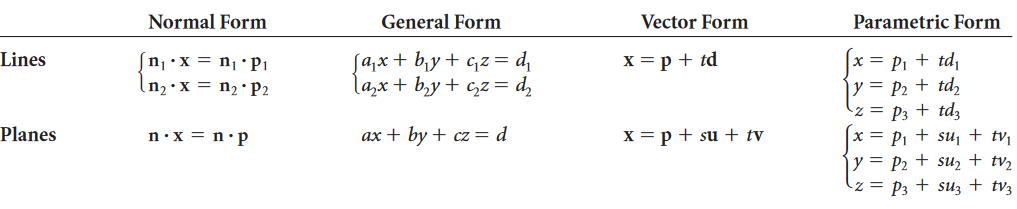
\includegraphics[scale=0.55]{example1-3-1.png}
\end{center}
\begin{enumerate}
    \item[] $d(B,l)=\cfrac{ax_0+by_0-c}{\sqrt{a^2+b^2}}$
    \item[] $d(B,P)=\cfrac{ax_0+by_0+cz_0-d}{\sqrt{a^2+b^2+c^2}}$
\end{enumerate}

\section{Code Vectors and Module Arithmetic}

\subsection*{Example}
Let $\*{u} = [1,1,0,1,0]$ and $\*{v} = [0,1,1,1,0]$ be two binary vectors of
length 5. Find $\*{u\cdot v}$.

\subsection*{Solution}
The calculation of $\*{u\cdot v}$ takes place in , so we have
$$\*{u\cdot v}=1\cdot0+1\cdot1+0\cdot1+1\cdot1+\mathbb{Z}_2 0\cdot0=0+1+0+1+0=0$$